\chapter{Preliminary Measurements}
\label{sec:prem}
\section{Working Voltage for the Photomultipliers}
As a first step, the optimal working voltages for the photomultipliers (PMTs) have to be found.
Two PMTs were chosen for this measurement as a sample from the whole detector, \texttt{R10B} and \texttt{R20A}.
It is important to choose PMTs from different planes to make sure the measured signal is due to a 
particle crossing the detector. A schematic for the measuring circuit is shown in \autoref{fig:hvscematic}.\\
\begin{figure}
    \centering 
    \includegraphics[width=0.8\textwidth]{figures/hv.jpg}
    \caption{Schematic representation of the coincidence counting circuit for the PMTs. 
    The signal propagation is from left to right starting with the PMTs and their high voltage supply and ending with the scaler.}
    \label{fig:hvscematic}
\end{figure}
Only signals measured with both PMTs are taken into account. To determine these coincidences 
logic signals are needed and for this, discriminators with a threshold of $\SI{40}{mV}$ are used. 
They convert the analogous signals of each PMTs into NIM standard signals. Using a logic unit module, we get
the coincidences from the logic \texttt{AND} of both PMT signals. The NIM signals 
last for $\SI{40}{\ns}$ each so the signals do not have to arrive at the same time but within 
$\SI{40}{\ns}$ of each other because the muons arrive in the different planes at different times 
and not necessarily at the same distance from the PMTs. Furthermore, the PMTs may have different
delay times as well.\\
For the measurement, the \texttt{R10B} PMT works on a fixed high voltage of $\SI{775}{V}$ while the high voltage of 
\texttt{R20A} is varied from $\SI{700}{V}$ to $\SI{900}{V}$. Each measurement lasts $\SI{200}{s}$.
The taken data is shown in \autoref{fig:hv}. A plateau can be found with $\SI{875}{V}$ corresponding to the middle value 
of it. This value is used as a fixed value for the \texttt{R20A} PMT when the voltage of the \texttt{R10B}
PMT is varied in the same range of high voltages. The measurements for this PMT were each taken in $\SI{100}{s}$ due to 
time limitations.
The central value of the plateau for this PMT is $\SI{825}{V}$.
Both measurements were also stopped when the PMTs are operating in the discharge region due to the high voltage to avoid damaging the PMTs.\\

The results are shown in \autoref{fig:hvPMT1} and \autoref{fig:hvPMT2}. All uncertainties are obtained 
assuming a Poissonian distribution, meaning $\sigma \propto \sqrt{N}$, where $N$ is the number of
coincidences. Because the output of the high voltage sources can fluctuate, the central values of the plateaus, $\SI{875}{V}$ for the \texttt{R20A} PMT and 
$\SI{825}{V}$ for the \texttt{R10B} PMT, can be used as the optimal working voltages to ensure
a voltage output in the region of the plateau.

\begin{figure}
        \centering
        \begin{subfigure}[b]{0.48\textwidth}
        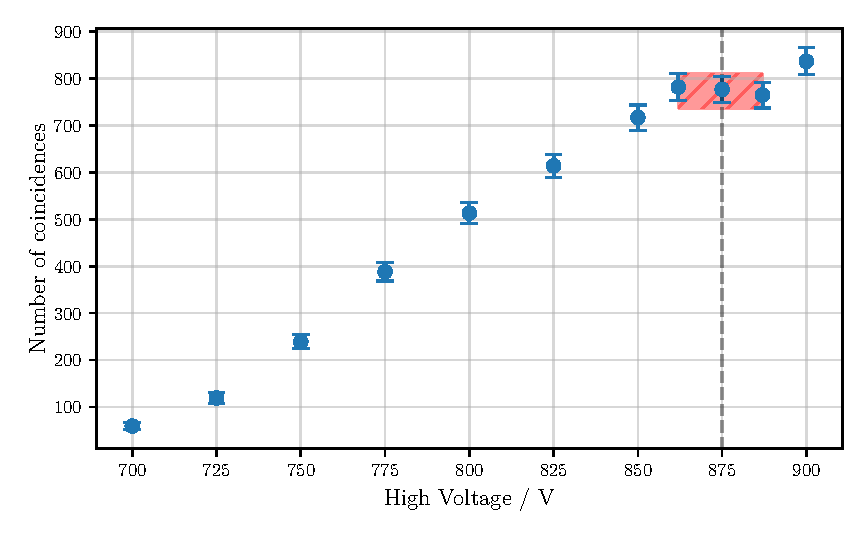
\includegraphics[width=\textwidth]{plots/hvR20A.pdf}
        \captionof{figure}{Data of the \texttt{R20A} PMT.
        The central value of the plateau is $\SI{875}{V}$.}
        \label{fig:hvPMT1}
    \end{subfigure}\hfill
\begin{subfigure}[b]{0.48\textwidth}
        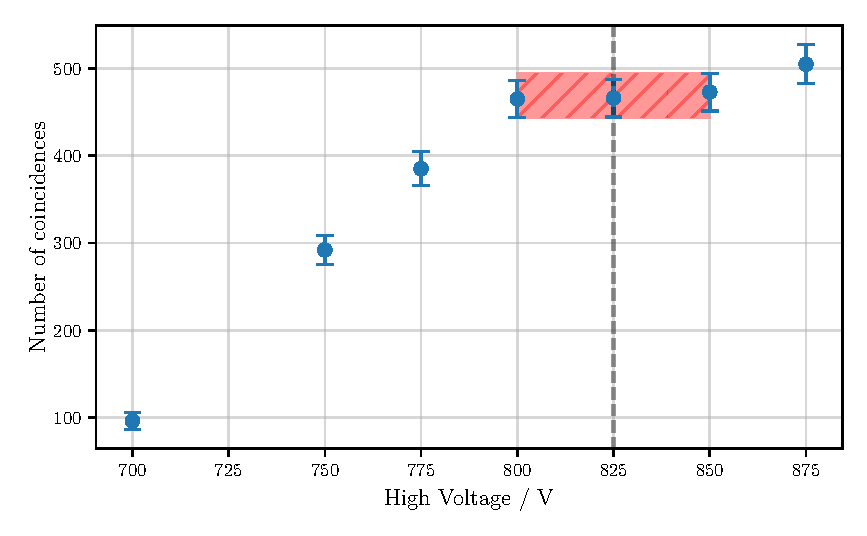
\includegraphics[width=\textwidth]{plots/hvR10B.pdf}
        \captionof{figure}{Data of the \texttt{R10B} PMT.
        The central value of the plateau is $\SI{825}{V}$.}
        \label{fig:hvPMT2}
\end{subfigure}
\caption{Measured number of coincidences regarding varying high voltages
of the \texttt{R10B} PMT and the \texttt{R20A} PMT.
The dashed line indicates the central values of each plateau. The striped red areas mark the found plateaus.}
\label{fig:hv}
\end{figure}
\section{Threshold measurements}
After the optimal working voltages was found, the determination of the optimal threshold voltage of the chosen PMTs started.
A good determination of the threshold is necessary to suppress electronic noise on the one hand, but also to make sure that real signals are not
filtered as well on the other hand. So the threshold can neither be too low nor too high.\\
 Similar to the step before, a counting experiment of coincidences concerning the threshold voltages is conducted. This time the circuit arrangement is shown in 
 \autoref{fig:threshold_scematic} is used. The PMTs are powered using the working voltages given 
 in the laboratory as an average optimal working voltage for three PMTs. \\
\begin{figure}
   \centering
   \includegraphics[width=0.87\textwidth]{figures/thresh.jpg}
   \caption{Schematic representation of the electronic circuit used to find the optimal threshold voltage
   .The signal flows from left to right, starting with the PMTs and Ending with the scaler.}
   \label{fig:threshold_scematic}
\end{figure}
In principle, the threshold of the discriminator of one plane is kept fixed at $\SI{15}{mV}$, while 
the threshold of the other discriminator is being varied from $\SI{5}{mV}$ to $\SI{250}{mV}$ in irregular steps. 
Using a discriminator and a Fan-in-Fan-out system as shown in \autoref{fig:threshold_scematic}, it is possible to vary the threshold of the discriminators of both PMT planes at the same time. Each counting measurement was conducted in $\SI{60}{s}$.\\ 
The results for the \texttt{R10} and \texttt{R20} planes can be seen in \autoref{fig:threshR10R20}.
Results from other planes have to be taken from \autoref{sec:appendix}, figures \autoref{fig:appthresh1} to \autoref{fig:appthresh6}.\\
\input{../content/treshtable.tex}
The data shows a higher number of coincidences at low threshold voltages, which decreases with rising voltages.
This behavior is the same for all PMTs although not all curves show it that clearly.  
Also, a plateau of optimal threshold voltages can be seen. From the middle of this plateau, a threshold voltage 
has to be chosen as the optimal threshold value. As before the uncertainties will be taken 
into consideration using the Poissonian error. The optimal threshold voltages of all PMTs are shown in 
\autoref{tab:thresh}.
Note that for the \texttt{L10} signals and the \texttt{R10} signals two measurements 
were taken. Thus, in these cases, only the value from the curve where it is easier to detect
where the plateau is will be taken into consideration.
The other values are marked italic in the tabular.
\begin{figure}
    \centering
    \begin{subfigure}[b]{0.48\textwidth}
    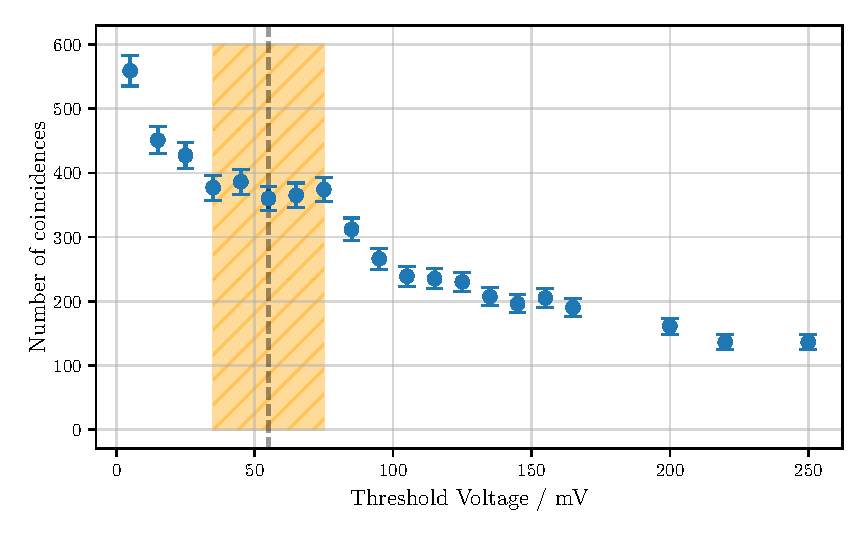
\includegraphics[width=\textwidth]{plots/threshR20.pdf}
    \captionof{figure}{Data of the \texttt{R20} PMTs.
    The central value of the plateau is $\SI{55}{mV}$.}
\end{subfigure}\hfill
\begin{subfigure}[b]{0.48\textwidth}
    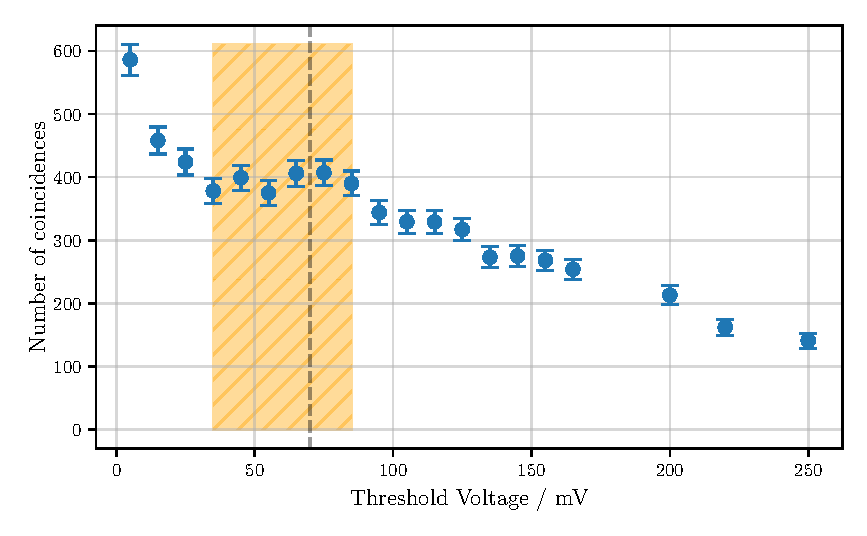
\includegraphics[width=\textwidth]{plots/threshR10.pdf}
    \captionof{figure}{Data of the \texttt{R10} PMTs.
    The central value of the plateau is $\SI{70}{mV}$.}
\end{subfigure}
\caption{Measured number of coincidences concerning varying threshold voltages
of the \texttt{R10} PMTs and the \texttt{R20} PMTs.
The dashed line indicates the central values of each plateau. The striped orange areas mark the found plateaus.}
\label{fig:threshR10R20}
\end{figure}
\section{TDC callibration}
